%\documentclass{beamer}
%\usetheme{Pittsburgh}
\documentclass{scrartcl}

\usepackage[utf8]{inputenc}
\usepackage{default}
\usepackage[procnames]{listings}
\usepackage{graphicx}
%\usepackage[toc,page]{appendix}
\usepackage{caption}
\usepackage{hyperref}
\usepackage{color}
%\usepackage{csvsimple}
\usepackage{float}
\usepackage[T1]{fontenc}



%Bibliogrpahy?
\usepackage{bibentry}
%\nobibliography*
%\bibentry{ }


%Python
\definecolor{keywords}{RGB}{255,0,90}
\definecolor{comments}{RGB}{0,0,113}
\definecolor{red}{RGB}{160,0,0}
\definecolor{green}{RGB}{0,150,0}
\lstset{language=Python,
    basicstyle=\ttfamily\scriptsize,
    keywordstyle=\color{keywords},
    commentstyle=\color{comments},
    stringstyle=\color{red},
    identifierstyle=\color{green},
    breaklines = true,
    columns=fullflexible,
    %Numbering and tabs
    %numbers=left,
    %numberstyle=\tiny\color{gray},
    %stepnumber=2,
    %numbersep=1em,
    tabsize=4,
    showspaces=false,
    showstringspaces=false}

\begin{document}

\title{Scientific Experimentation and Evaluation
}
\subtitle{
Assignment: 3.1}
\author{
  Matin, Maryam \\
  Quignon, Christophe
  %Familyname, Name
}
\date{\today}


\maketitle


\section{Design Report}

\subsection{Calibration Setup}
\paragraph{Description}

In this exercise we aim to calibrate a camera using some image patterns.

In order to minimize the full distortion of the images received from the camera we need to have some distortion corrections regarding both radial and tangential distortions. For this goal we will set our camera at a fixed position and capture several still images of a printed checkerboard pattern from different orientations and translations with respect to the camera. we will then calculate all the intrinsic and extrinsic parameters of the camera to extract undistorted images. 

Zhang\cite{zhang}  introduces a new approach for camera calibration. Using his approach for a successful calibration we only need a few ( at least 2) pattern images. The internal camera model in the Mathlab toolbox for camera calibration is very similar to the one introduced by Heikkil \cite{heikkila}. In our experiments we will be using the OpenCV library of the similar toolbox using python. Using this toolbox one needs at least 10 image patterns. So for this experiment we decided to capture at least 20 image patterns from different angles We start with an orthogonal view and then two rotations with roughly 30 degrees on every axis of the frame and also from different distances from the camera.

The code was implemented in python. The images are first converted to grayscale and then the corners and the dimensionality of the checkerboard is given. We will use and 8*8 checkerboard that with 20 mm length. The calibration stage is then done and we iterate the same steps until the errors are small enough or we reach a certain number of iterations.


The tangential distortion is a manufacturing issue and  is due to imperfect alignment of the lens in the center of the camera. It is observed that in todays cameras this distortion is usually such small that we can simply neglect.



\paragraph{Possible errors}
\begin{itemize}
\item If the distortion is high, it is possible that the extracted corners by the toolbox don't fit the real image corners. To solve this issue as suggested in [3 ], we can improve the corner extraction by entering an initial guess of the lens distortion coefficient which is a number between -1 and 1 and repeat it until the extracted corners are satisfactory.

%\href{http://www.vision.caltech.edu/bouguetj/calib_doc/htmls/example.html...}{vision.caltech.edu/bouguetj/calib\_doc/htmls/example.html...}  


\item Another issue which may happen if the distortion is high, is that the program might not be able to detect the number of squares automatically. In this case we should enter the numbers manually.

\item We can use the error plot to see how large the reprojection error is. Large error for a large number of images demonstrates that the corner extraction phase was not accurate enough and therefore we need to enhance that step by adding the predicted distortion option.

\end{itemize}

\paragraph{Pitfalls}
\begin{itemize}
\item Lighting conditions can make the pattern indistinguishable
\item The camera frame must not move
\item The calibration pattern may be scaled or even distorted during the printing procedure
\item The calibration pattern must be flat and not curved
\item The background must not contain patterns similar to the calibration pattern
\item When the captured imaged is stored, compression should not distort the calibration pattern
\item The lens has to be clean
\end{itemize}


\subsection{Image estimation}
\paragraph{Number of images}
%Zhang\cite{zhang} stated a method that works with at least two different orientations.

For the testrun, we user 20 images from the camera calibration toolbox that can be downloaded under \href{http://www.vision.caltech.edu/bouguetj/calib_doc/htmls/calib_example.zip}{vision.caltech.edu/bouguetj/calib/\_doc/htmls/calib\_example.zip}

\paragraph{Image positions}
%Either the image or the camera can be freely moved and the movement need not be known. (Zhang\cite{zhang}).
%We start with an orthogonal view and then two rotations with roughly 30 $^\circ $ on every axis of the frame.


\subsection{Parameter description}

\paragraph{Parameter description}
\begin{itemize}
\item ret\\
Is True if the pattern is found in the image.

\item mtx\\
Is the Output 3x3 floating-point camera matrix which contains information of the Focal length and the Principal point.The component on the last row and last column is set to 1.
It depends on the camera only, so once calculated, it can be stored for future purposes.
\item dist\\
Is the 1x5 distortion coefficients matrix.
\item rvecs\\
Output vector of rotation vectors estimated for each pattern view. That is, each k-th rotation vector together with the corresponding k-th translation vector brings the calibration pattern from the model coordinate space to the world coordinate space.
\item tvecs\\
Output vector of translation vectors estimated for each pattern view.
\item newcameramtx\\
The optimal new camera matrix based on the free scaling parameter. The resulting image may include some black pixels corresponding to “virtual” pixels outside of the captured distorted image.
\item roi\\
Reigon of interest for cropping the image to get the best undistorted image.
\end{itemize}

\paragraph{Parameter output}
(See last.out)
\lstinputlisting{last.out}

\subsection{Possible Problems}
%\paragraph{Calibration}
%Error sources


\begin{figure}[H]
\centering
\begin{minipage}{.5\textwidth}
  \centering
  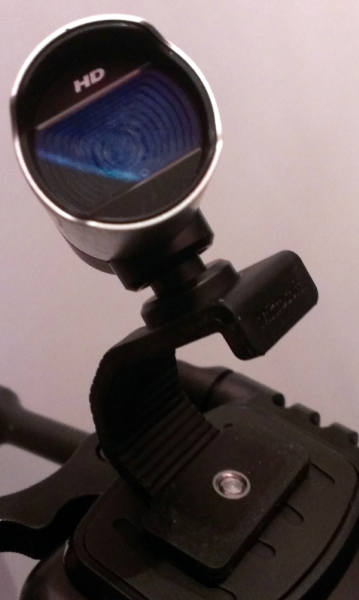
\includegraphics[width=.8\linewidth]{img/rotation.jpg}
  %\caption{}
  %\label{fig:}
\end{minipage}%
\begin{minipage}{.5\textwidth}
  \centering
  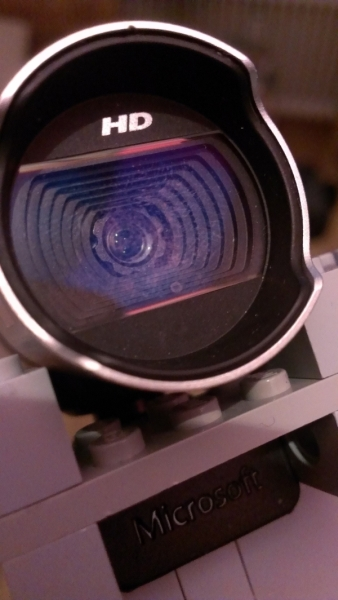
\includegraphics[width=.8\linewidth]{img/lense.jpg}
  %\caption{}
  %\label{fig:} 
\end{minipage}
\caption{Rotation on the tripod (left) and a dirty aperture (right) are source of possible errors.}
\label{fig:errorsources}
\end{figure}
%TODO DESCRIPTION



\begin{figure}[H]
\centering
\begin{minipage}{.5\textwidth}
  \centering
  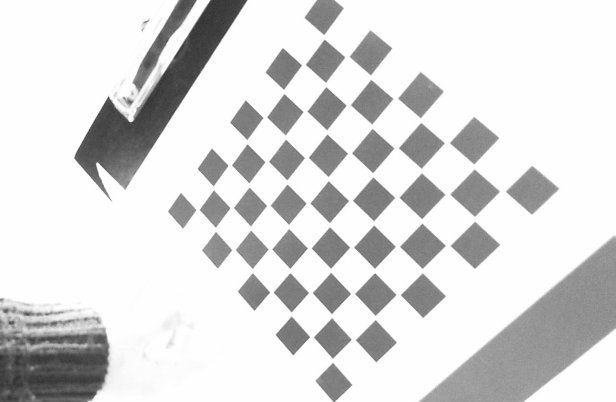
\includegraphics[width=.8\linewidth]{img/brightness.jpg}
  %\caption{}
  %\label{fig:}
\end{minipage}%
\begin{minipage}{.5\textwidth}
  \centering
  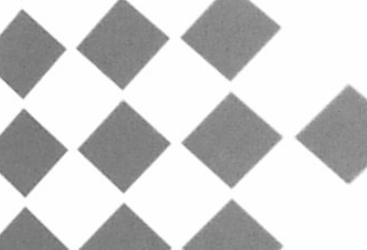
\includegraphics[width=.8\linewidth]{img/bright_detail.jpg}
  %\caption{}
  %\label{fig:} 
\end{minipage}
\caption{An image taken (left) including detail view (right) with too high brightness}
\label{fig:brightness}
\end{figure}
%TODO DESCFRIPTION



%\paragraph{Experiment}
%problems while testing including problems with laptop/camera

%The camera connected without any issues
%It is important to release the camera after taking an image, otherwise it will stay blocked
%One has to make sure which index to use, because the index destinguished between the built-in camera of the laptop and the usb camera
%The camera is very light sensitive. It works best at low light.


\begin{figure}[H]
\centering
\begin{minipage}{.5\textwidth}
  \centering
  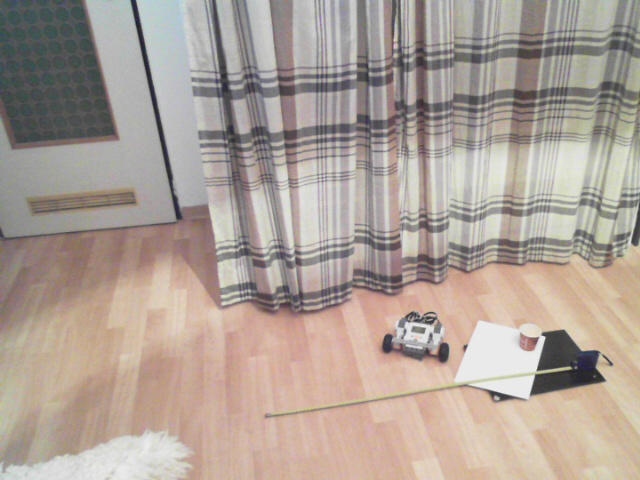
\includegraphics[width=.8\linewidth]{img/testimgbad.jpg}
  %\caption{}
  %\label{fig:}
\end{minipage}%
\begin{minipage}{.5\textwidth}
  \centering
  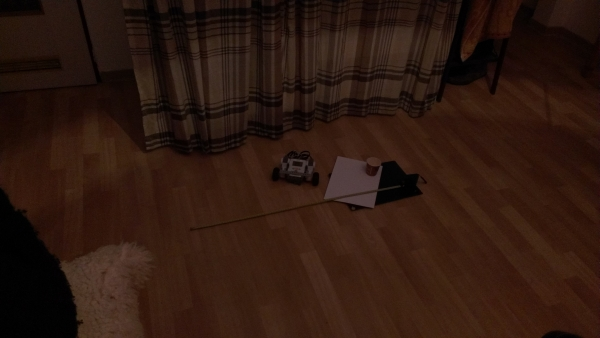
\includegraphics[width=.8\linewidth]{img/iso400.jpg}
  %\caption{}
  %\label{fig:} 
\end{minipage}
\caption{The camera is very light sensitive (left) in comparison to digital ISO 400 (right). In both images the background could disturb the calibration pattern.}
\label{fig:brightness}
\end{figure}
%TODO DESCRIPTION



%maybe we exclude this
\section{Appendix}

\subsection{Example images}

\begin{figure}[H]
\centering
\begin{minipage}{.5\textwidth}
  \centering
  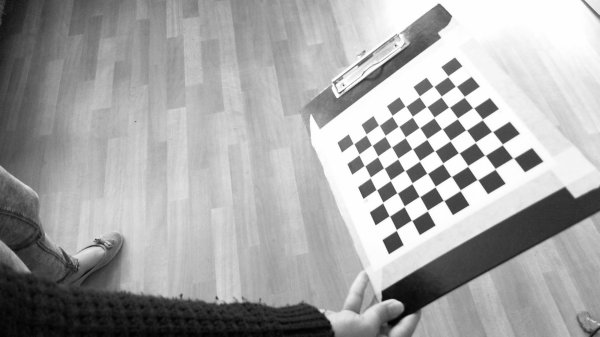
\includegraphics[width=.8\linewidth]{img/cap_18.jpg}
  %\caption{}
  %\label{fig:}
\end{minipage}%
\begin{minipage}{.5\textwidth}
  \centering
  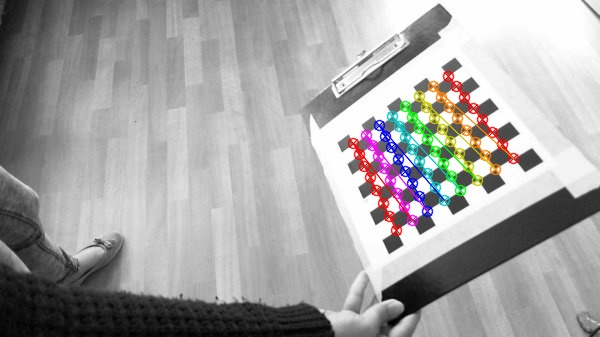
\includegraphics[width=.8\linewidth]{img/cap_18_corners.jpg}
  %\caption{}
  %\label{fig:} 
\end{minipage}
\caption{One of the images taken and the according corners. (resized)}
\label{fig:output}
\end{figure}

%TODO DESCRIPTION


\subsection{cam2jpg.py}
\lstinputlisting[language=Python]{cam2jpg.py}


\subsection{calibration.py}
\lstinputlisting[language=Python]{calibration.py}




%BIBLIOGRPAHY!
\bibliographystyle{plain}%amsalpha
\bibliography{bib.bib}
%\bibentry{}


%COPY AND PASTE FROM HERE

%\begin{enumerate}
% \item
%\end{enumerate}

%\href{link}{text}

%\begin[Language=Python]{lstlisting}
%#PYTHON CODE HERE
%\end{lstlisting}

%\lstinputlisting[language=Java]{ }

%\csvautotabular[separator=semicolon]{data.csv}

%\begin{figure}
% \center
% \includegraphics[width= cm]{img/ }
% \caption{}
%\end{figure}



\end{document}
